\documentclass[tikz]{standalone}
\usetikzlibrary{calc,trees,positioning,arrows,chains,shapes.geometric,%
    decorations.pathreplacing,decorations.pathmorphing,shapes,%
    matrix,shapes.symbols,fit}

\pgfdeclarelayer{back}
\pgfsetlayers{back,main}


\makeatletter
\tikzset{
  fitting node/.style={
    inner sep=0pt,
    fill=none,
    draw=none,
    reset transform,
    fit={(\pgf@pathminx,\pgf@pathminy) (\pgf@pathmaxx,\pgf@pathmaxy)}
  },
  reset transform/.code={\pgftransformreset}
}
\makeatother


\begin{document}
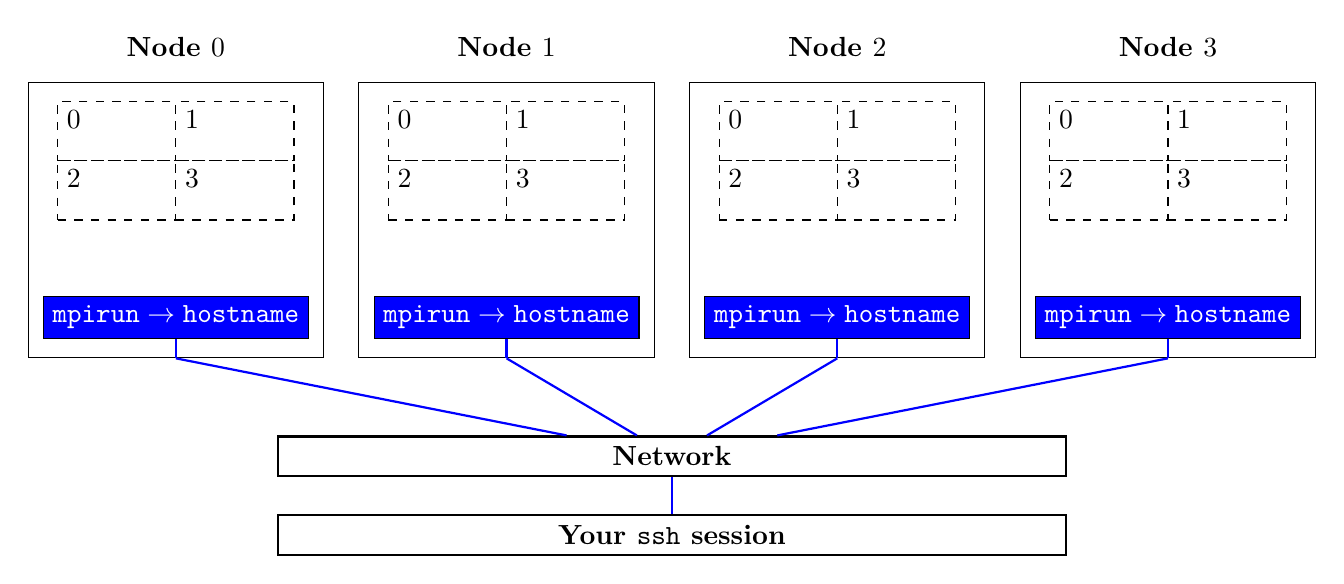
\begin{tikzpicture}

  \node [draw,thick,rectangle, minimum width=10cm, minimum height=.5cm] at($(1.5*4.2,0)$) (switch) {\bfseries{}Network};
  \node [draw,thick,rectangle, minimum width=10cm, minimum height=.5cm] at($(1.5*4.2,-1)$) (you) {\bfseries{}Your \texttt{ssh} session};
  \path [thick,color=blue] (switch) edge (you) ;
  
  \foreach \n in {0,...,3}
  {
   
    \node [draw,rectangle, minimum width=3.75cm, minimum height=3.5cm] at($(0,3)+(4.2*\n,0)$) (node_\n) {};
    \node [node distance=2mm,above =of node_\n] (node_label_\n) {\bfseries{}Node $\n$};
    \node (anchor_for_cores_\n) at($(node_\n)+(0,.75)$)  {};

    \begin{scope}[every node/.style={draw, %
        dashed,%
        rectangle, %
        on grid, %
        minimum height=.75cm,%
        minimum width=1.5cm, 
        node distance=3.75mm and 7.5mm%
      }]
      \node [above left =of anchor_for_cores_\n] (node_\n_cpu_0) {};
      \node [above right=of anchor_for_cores_\n] (node_\n_cpu_1) {};
      \node [below left =of anchor_for_cores_\n] (node_\n_cpu_2) {};
      \node [below right=of anchor_for_cores_\n] (node_\n_cpu_3) {};
    \end{scope}
    \foreach \c in {0,...,3}
    {
      \node [below right] at(node_\n_cpu_\c.north west) {$\c$};
    }
    
    % \draw[thick] (node_\n.south) -- (switch)  {};

    \node [draw, above, fill=blue, text=white] at($(node_\n.south)+(0,.25)$) (mpirun_call_\n) {$\texttt{mpirun} \rightarrow \texttt{hostname}$};
    \path [thick,color=blue] (mpirun_call_\n) edge (node_\n.south) 
    (node_\n.south) edge (switch);
  }



\end{tikzpicture}
\end{document}
